\documentclass{standalone}

\usepackage{tikz}

\begin{document}
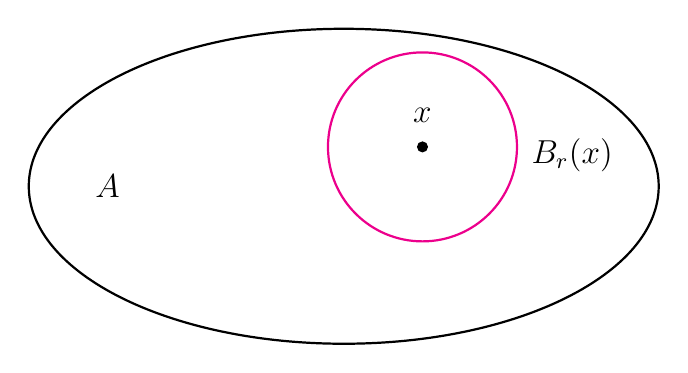
\begin{tikzpicture}
  % Draw the ellipse A
  \draw[thick] (0,0) ellipse (4cm and 2cm);
  \node at (-3,0) {\large$A$};
  
  % Center of the ball x
  \fill (1,0.5) circle (2pt);
  \node at (1,0.9) {\large$x$};
  
  % Draw the ball B_r(x)
  \draw[magenta, thick] (1,0.5) circle (1.2cm);
  \node at (2.9,0.4) {\large$B_r(x)$};
\end{tikzpicture}
\end{document}
